\section{Technical Difficulties}
\label{sec:tech-diff}

\subsection{Creating the Mammogram image data}

As this project was building upon the work done by Learned-Miller \cite{joint-alignment}, it was useful to utilise the load function that was already in place. However, the nature in which the image files were loaded into the system caused some unexpected hurdles.

In order to understand how the demo data was uploaded, and therefore implement a function to compile a large set of \gls{mammographic images} in the correct format, research was carried out into the nature of \acrshort{pgm} files, and the function which comments play in the headers.

\subsubsection{PGM file format}

\acrfull{pgm} file format is part of a package called Netpbm, which contains 220 separate programs for dealing with files such as \acrshort{pgm}, pbm and pnm. As the name suggests, it is a lightweight-greyscale image format, which is simple for use in programs, making it ideal for this project.

The structure of \acrshort{pgm} files is very specific and is defined as \cite{PGM_Format}:

\begin{figure}[H]
  \begin{minted}
  [
  %gobble=2,
  xleftmargin= 0.5cm,
  numberblanklines=true,
  numbersep=12pt,
  numbersep=5pt,
  gobble=0,
  frame=leftline,
  breaklines,
  %frame=lines,
  %framesep=2mm,
  baselinestretch=1.2,
  fontsize=\small,
  linenos
  ]
  {text}
  A `magic number' which identifies the file type. A pgm image's magic number is the two characters `P5'.
  Whitespace (in the format of tab, space etc)
  A width, formatted as ASCII characters in decimal.
  Whitespace (in the format of tab, space etc)
  A height (in the same format as width)
  Whitespace (in the format of tab, space etc)
  Maximum Grey Value (Maxval) - usually 255
  Single whitespace character (typically new line)
  A raster of Height rows, in order from top to bottom. Each row consists of Width gray values, in order from left to right. Each gray value is a number from 0 through Maxval, with 0 being black and Maxval being white. Each gray value is represented in pure binary by either 1 or 2 bytes. If the Maxval is less than 256, it is 1 byte. Otherwise, it is 2 bytes. The most significant byte is first.
  \end{minted}
  \caption{PGM header rules}
  \label{fig:pgm-header-rules}
\end{figure}

A comment in \acrshort{pgm} is proceeded by the \# symbol, and is not counted in the formatting as defined in Figure \ref{fig:pgm-header-rules}.

\subsubsection{Specific file format for \Gls{Congealing}}
\label{sssec:load}

 When investigating the \Gls{Congealing} demo code, it became apparent that comments were utilised in the reading-in of image information.

 \begin{figure}[H]
   \begin{minted}
   [
   xleftmargin= 0.5cm,
   numberblanklines=true,
   numbersep=12pt,
   numbersep=5pt,
   gobble=0,
   frame=leftline,
   breaklines,
   %frame=lines,
   framesep=2mm,
   baselinestretch=1.2,
   fontsize=\small,
   linenos
   ]
   {text}
P5
# 28 28 6742
2324 2324
255
  \end{minted}
\caption{Example MNIST PGM file header}
\label{fig:pgm_header_written}
\end{figure}


Figure \ref{fig:pgm_header_written} above shows the first five lines of the \acrshort{pgm} MNIST data which was included in the \Gls{Congealing} demo. The second line, proceeded by a \#, therefore a comment, includes information on height and width of each individual MNIST number (28 and 28), and how many of these numbers are included in the large file (6742).

This information is then used to set the number of images per row and to set an array to the appropriate height, width and number of included images in the \texttt{loadSeries.m} function.


\subsubsection{Creating an appropriate save function}

The next step was to write a function which would appropriately concatenate the mini-MIAS dataset \cite{Suckling_1994} to create a large \acrshort{pgm} input image for \Gls{Congealing}. This led to the function \\ \texttt{pgm2bigPgm.m}, which is a pre-processing funciton before the original \texttt{saveSeries.m} demo function, which will:
\begin{itemize}
\item read in the number of images in the chosen directory
\item identifies the dimensions of each scan in the directory (with mini-MIAS, they are all the same dimensions)
\item creates a string containing all the suitable information needed for reading (as outlined in Subsubsection \ref{sssec:load})
\item creates a file called \texttt{big\_scan.pgm} and saves all the images out to the one file (after transposition, as in Subsection \ref{ssec:trans})
\end{itemize}

\subsubsection{Final outcome}

An example of the final mammogram image data can be found in Figure \ref{fig:final-output-4}. When the user specifies an odd number of images, or the number of images do not create a square, extra black padding is created around the image, as can be observed in Figure \ref{fig:all-input-imgs}. There was an issue with the images rotation 90{\degree} as will be covered in the next Section.


\subsection{Image Rotation}
\label{ssec:trans}

One issue which was faced when creating the large .pgm file containing all the input images was that they were rotated 90{\degree} to the right, as demonstrated in Figure \ref{fig:rotated-input}.

\begin{figure}[H]
  \centering
  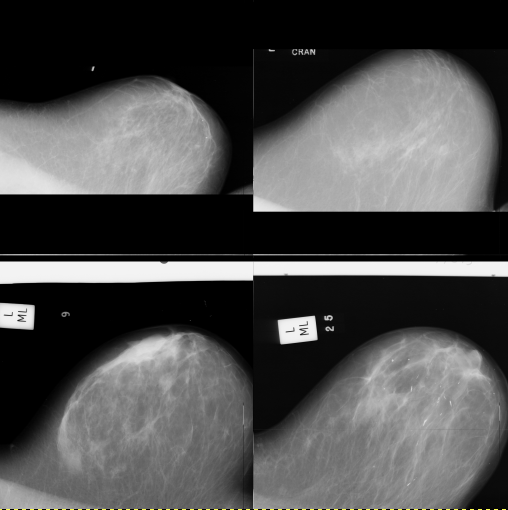
\includegraphics[width=0.4\textwidth]{Chapter2/technical-img/rotation.png}
  \caption{Four rotated input images concatenated into one larger image.}
  \label{fig:rotated-input}
\end{figure}

It quickly became apparent that the order in which the image array was being written to file to create this larger pgm file was incorrect, however due to MATLAB's use of vectorisation, it was difficult to diagnose where the issue lay. After some investigation, it was revealed that the function \texttt{fwrite} by MATLAB \cite{fwrite}, used for writing binary data to file, wrote each line out column-by-column, rather than the customary row-by-row approach.

To mitigate this issue, the array would have to be transposed prior to or during being passed into \texttt{fwrite}. There are two ways in which MATLAB permits the \gls{transposition} of arrays:

\subsubsection{Simple 2D array transposition}

MATLAB has a `Transpose' function \cite{transpose} which simply swaps the row and column values in a 2D array as utilised in:

\begin{minted}
  [
  xleftmargin= 0.5cm,
  numberblanklines=true,
  numbersep=12pt,
  numbersep=5pt,
  gobble=0,
  frame=leftline,
  breaklines,
  framesep=2mm,
  baselinestretch=1.2,
  fontsize=\small,
  %linenos
  ]
  {matlab}
fwrite(output,handles.finalImg.','uchar');
\end{minted}

Where handles.finalImg is a GUI holder for a 2D array of pixel values. This example was taken from the \texttt{removeMarker.m}  function - where the user can remove medical markers and save the output back to the original file.

\subsubsection{3D+ array transposition}

For arrays with more than 2 dimensions, simply swapping the values around will not work, so the MATLAB function \texttt{permute} \cite{permute} must be used.

\begin{minted}
  [
  xleftmargin= 0.5cm,
  numberblanklines=true,
  numbersep=12pt,
  numbersep=5pt,
  gobble=0,
  frame=leftline,
  breaklines,
  framesep=2mm,
  baselinestretch=1.2,
  fontsize=\small,
  linenos
  ]
  {matlab}

sers=zeros(squareImageSize(1),squareImageSize(2),noOfScans); %set size of array

for i = 1:noOfScans

  scan = fopen(strcat(pathname,'/',scanDirectory(i).name)); %open each input image individually
  im=(fread(scan,[squareImageSize(1),squareImageSize(2)],'uchar'));
  sers(:,:,i) = im; %add each input image to a 3D array which compiles all the input images into one

end

outfname=sprintf('%s/big_scan.pgm', pathname);
s=sers(:,:,:);
saveSeries(outfname,permute(s,[2,1,3])); %use the saveSeries demo function to write the final image arrays out to a file

\end{minted}

This example was taken from the \texttt{pgm2bigPgm.m} function - where a set of input images are passed in, and a large pgm image containing all the input images is outputted (as in Figure \ref{fig:final-output-4}). This image is then passed into the \Gls{Congealing} algorithm for alignment.

\subsubsection{Final Outcome}

After transposing all arrays which are to be saved out to file, whether directly through \texttt{fwrite} or via the \texttt{saveSeries} function, all images are saved in the correct orientation.

\begin{figure}[H]
  \centering
  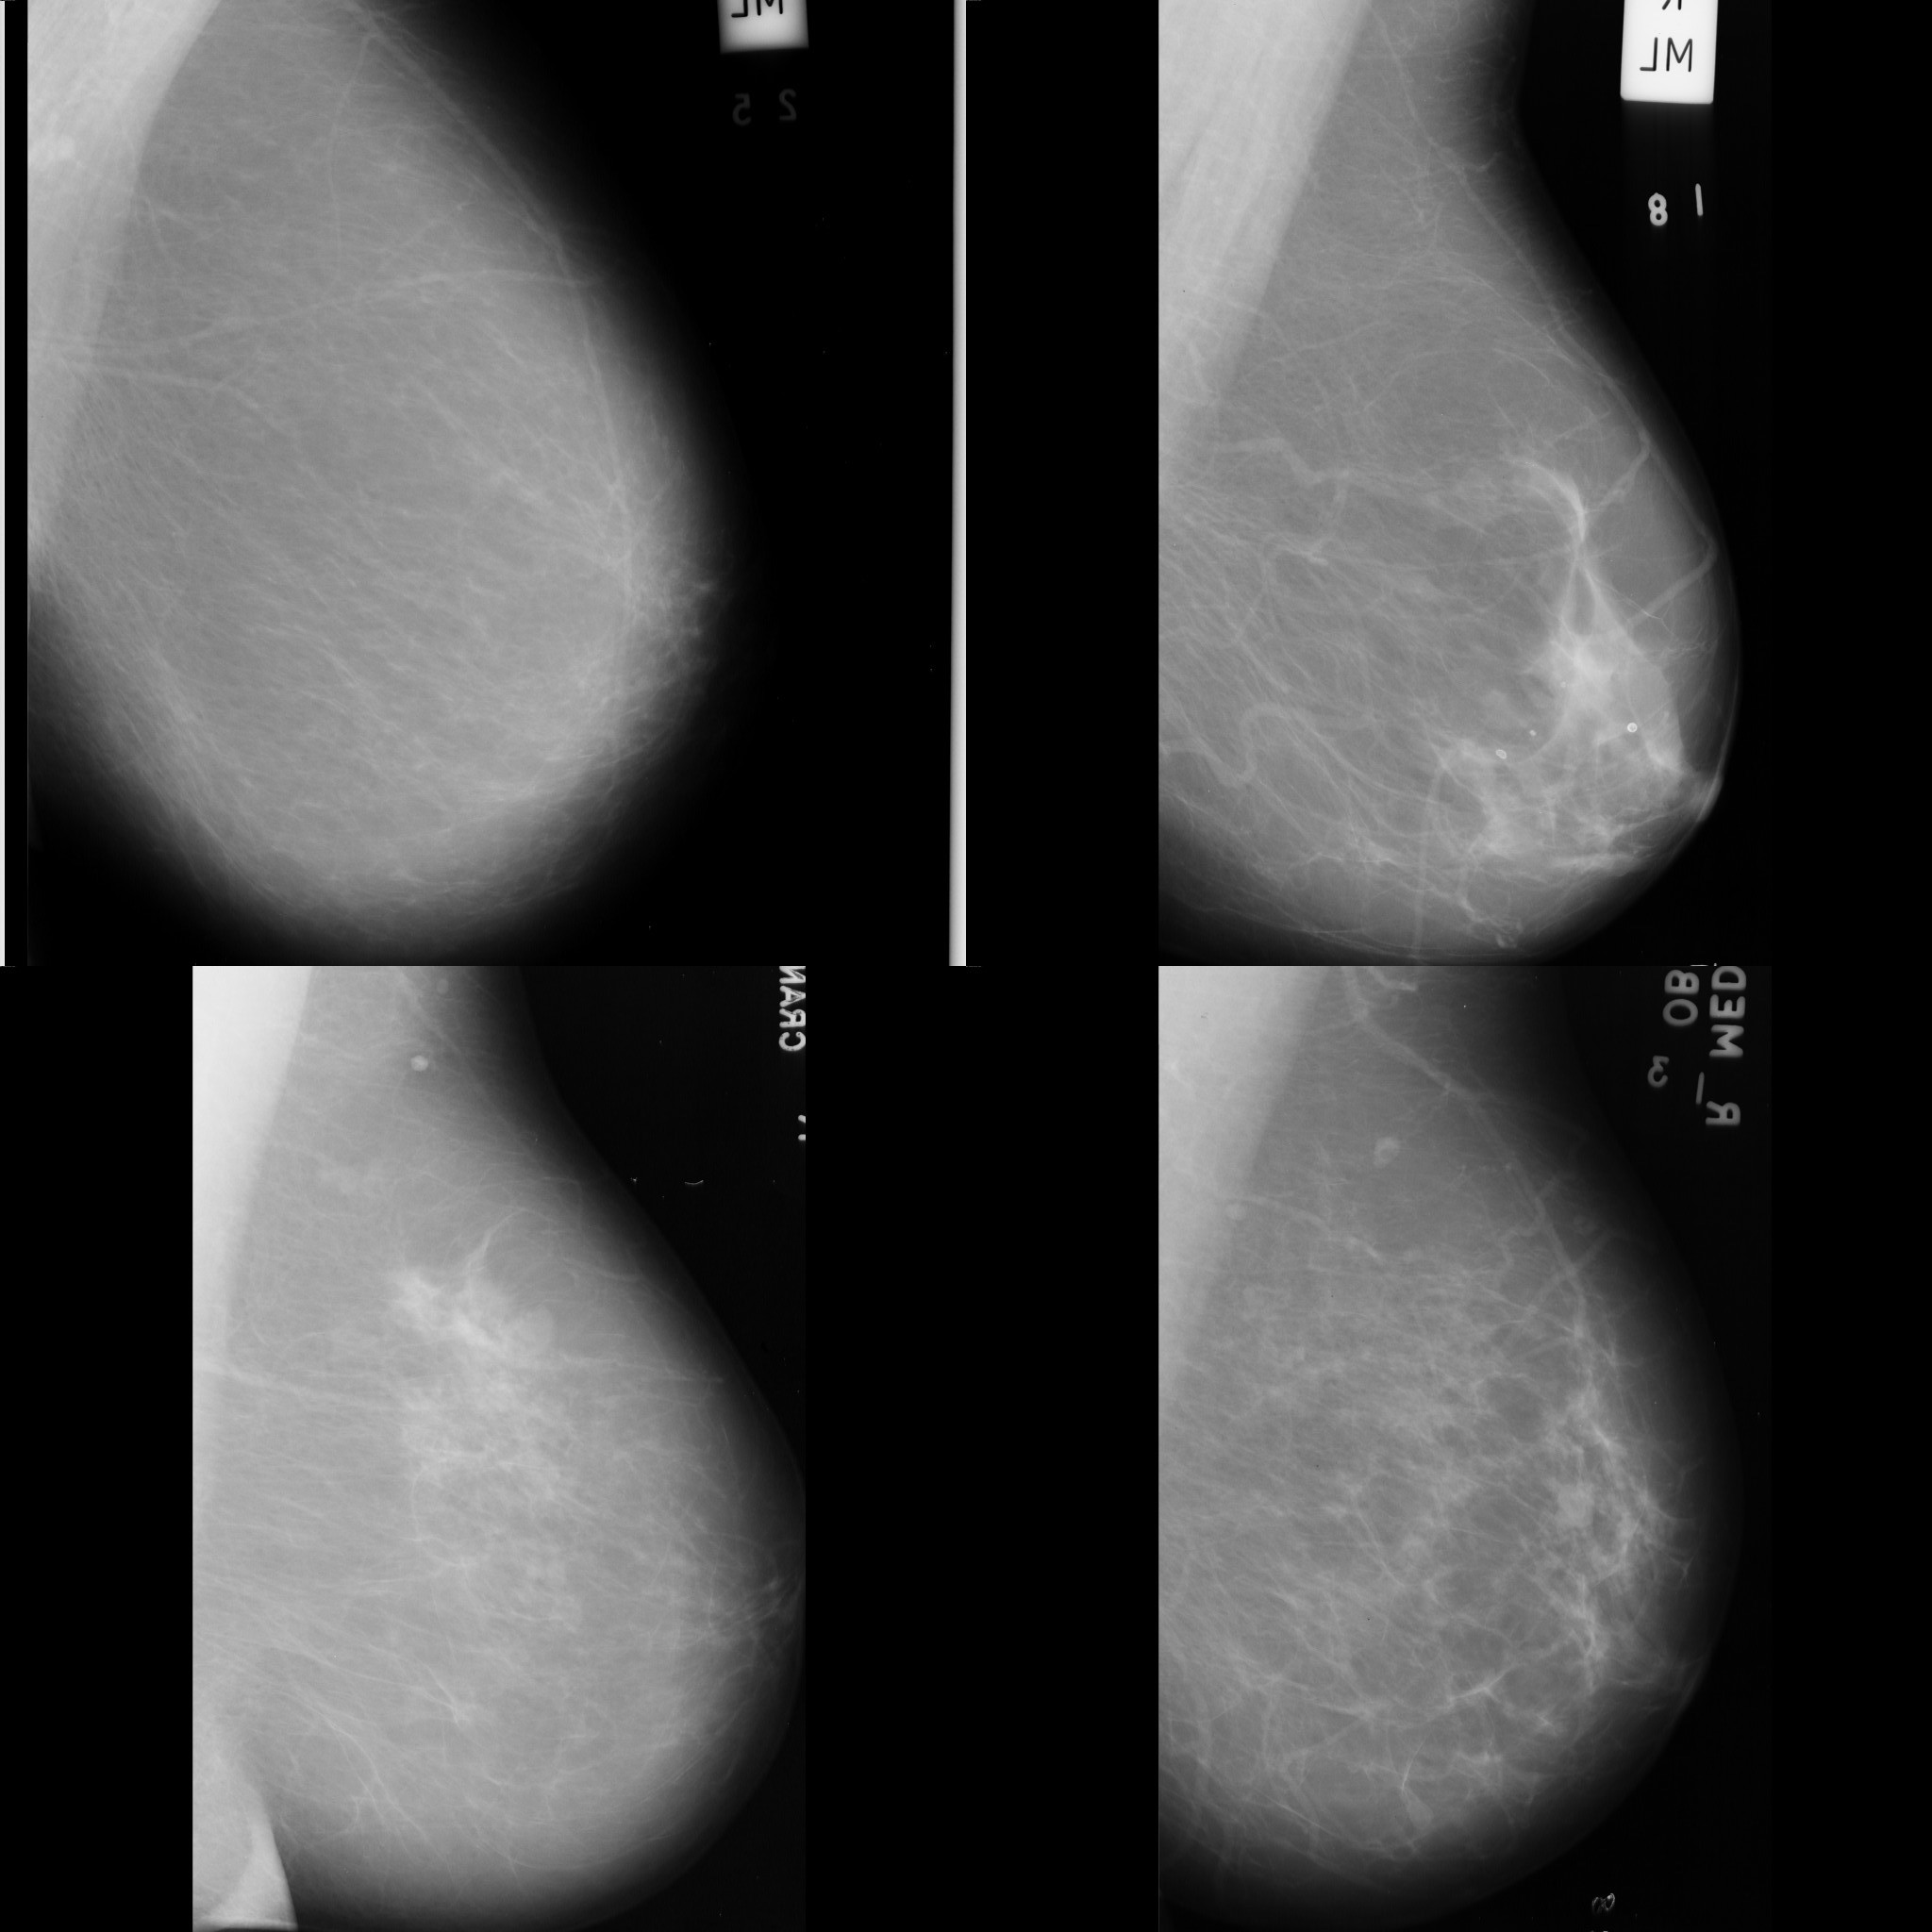
\includegraphics[width=0.3\textwidth]{Chapter2/technical-img/big_scan.jpg}
  \caption{Final output image.}
  \label{fig:final-output-4}
\end{figure}

\subsection{Medical Marker Removal}
\label{ssec:marker-removal}

This subsection has been formalised from a blog post written by the author on 28th March 2016 \cite{Collins_2016}.

As the images are aligned using a comparison of the pixel-value, the medical markers included on mammograms cause an issue. This is because if more than one scan contains these white patches (left by the metal clip during scanning), then they will try and align with each other during the \Gls{Congealing} process.

\begin{figure}[H]
  \centering
  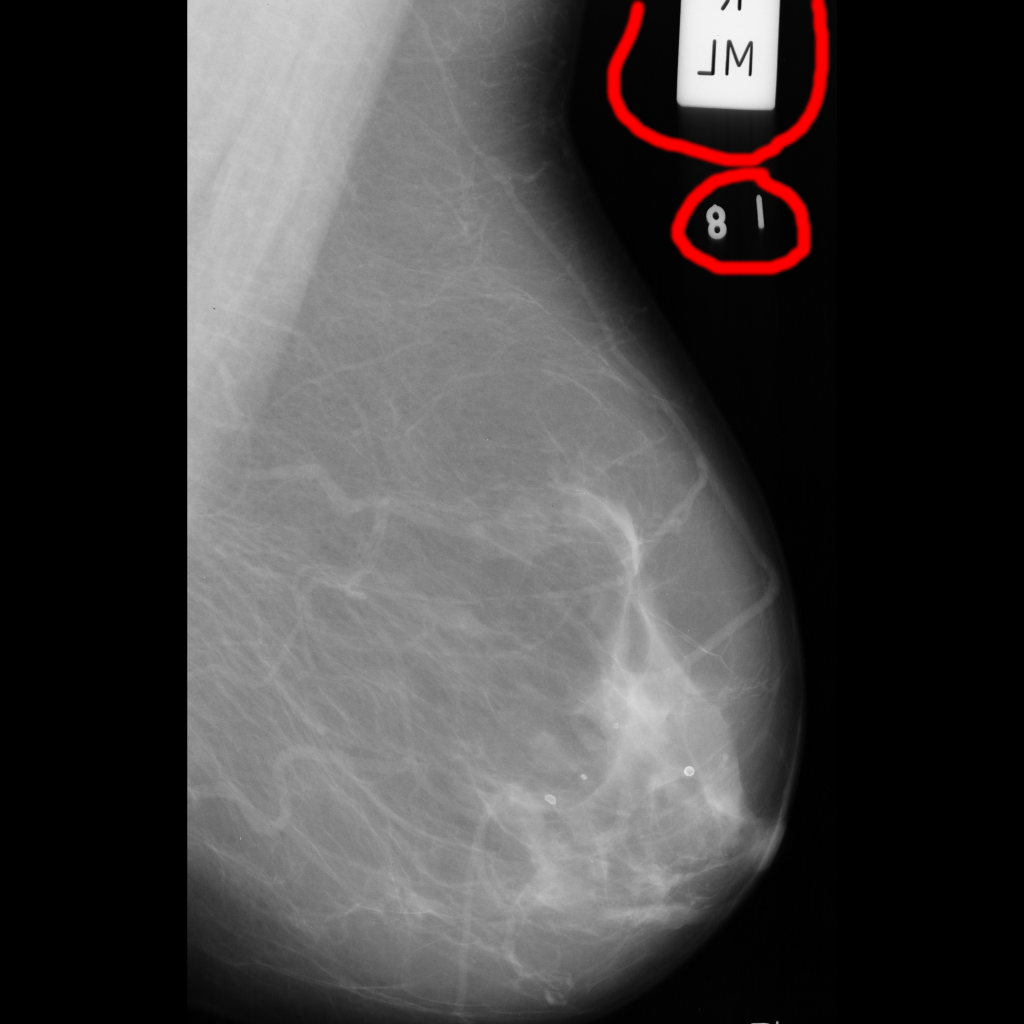
\includegraphics[width=0.4\textwidth]{Chapter2/technical-img/mdb196.png}
  \caption{Image containing medical markers}
  \label{fig:med-markers}
\end{figure}

Two options were available for the avoidance of medical markers:
\begin{itemize}
  \item Ask the user not to use images containing medical markers
  \begin{itemize}
    \item This is extremely restrictive
    \item This could massively reduce their number of usable images
  \end{itemize}
  \item Find a computer vision and/or image processing technique to remove these clips
  \begin{itemize}
    \item Preferably automatically
    \item Manually removing would work for small input data sets
  \end{itemize}
\end{itemize}

The following subsection will discuss the discarded ideas explored for artefact removal, before moving on to discuss the final implemented solution.

\subsubsection{Discarded ideas}

\begin{figure}[H]
    \centering
    \begin{subfigure}[t]{0.3\textwidth}
        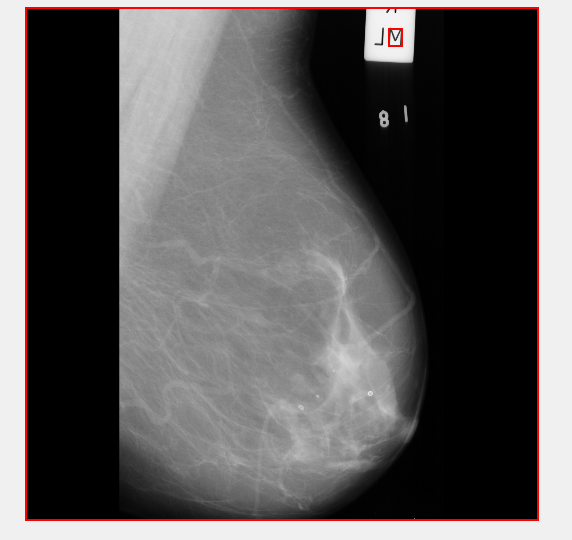
\includegraphics[width=\textwidth]{Chapter2/technical-img/morph.png}
        \caption{Squares detected in a mammogram using morphological operations.}
        \label{fig:morph}
    \end{subfigure} \hfill
    ~ %add desired spacing between images, e. g. ~, \quad, \qquad, \hfill etc.
      %(or a blank line to force the subfigure onto a new line)
    \begin{subfigure}[t]{0.3\textwidth}
        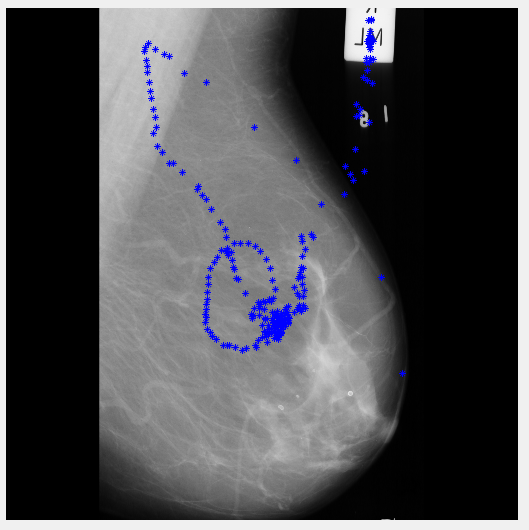
\includegraphics[width=\textwidth]{Chapter2/technical-img/regionprops.png}
        \caption{Regionprops detecting areas and superimposing the area information on a mammogram.}
        \label{fig:regionprops}
    \end{subfigure} \hfill
    \begin{subfigure}[t]{0.3\textwidth}
      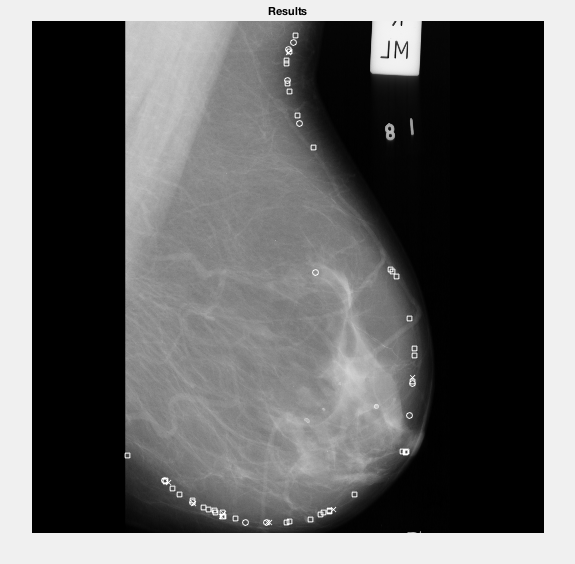
\includegraphics[width=\textwidth]{Chapter2/technical-img/shape_recog.png}
      \caption{Shape recognition picking out the rough boundary of breast tissue.}
      \label{fig:shape-recog}
    \end{subfigure}
    ~ %add desired spacing between images, e. g. ~, \quad, \qquad, \hfill etc.
    %(or a blank line to force the subfigure onto a new line)

    \begin{subfigure}[t]{0.3\textwidth}
      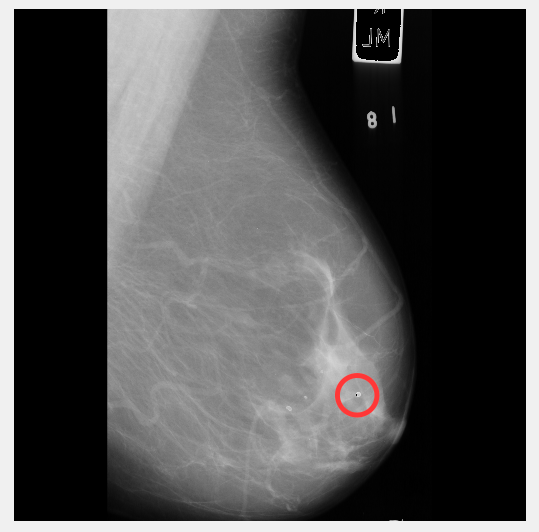
\includegraphics[width=\textwidth]{Chapter2/technical-img/remove-white-220.png}
      \caption{Removing areas of grey-level value above 220.}
      \label{fig:remove-white}
    \end{subfigure} \hfill
    \begin{subfigure}[t]{0.3\textwidth}
      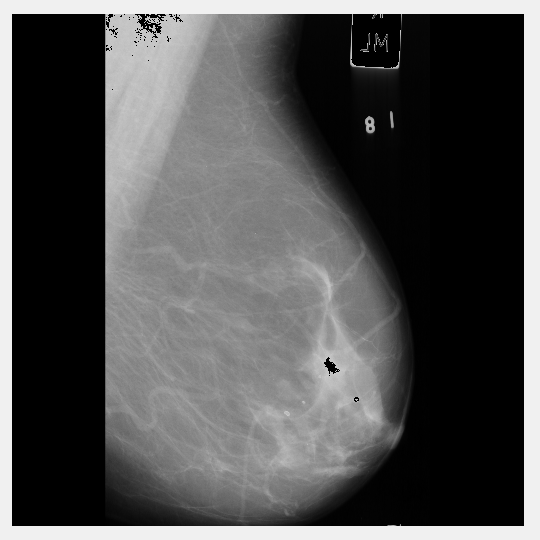
\includegraphics[width=\textwidth]{Chapter2/technical-img/remove-white.png}
      \caption{Lower grey-level removal threshold to 200.}
      \label{fig:remove-white-200}
    \end{subfigure} \hfill
    \begin{subfigure}[t]{0.3\textwidth}
      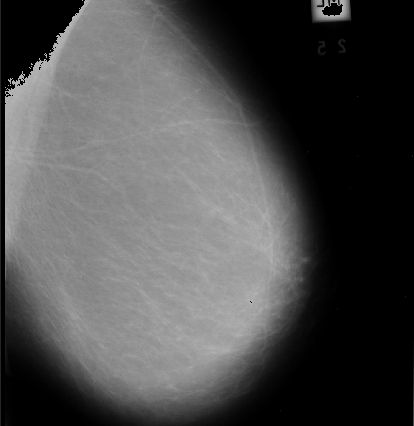
\includegraphics[width=\textwidth]{Chapter2/technical-img/other-scan.png}
      \caption{Applying removal over 220-value to another scan.}
      \label{fig:remove-other-scan}
    \end{subfigure}
    \caption{Output of discarded methods of marker removal}
    \label{fig:marker-removal-discards}
\end{figure}

\noindent \textbf{Morphological operation - remove squares from image}

Utilising a morphological operation, such as the one demonstrated by Chandra Kurniawan in the thread \cite{detect_square} was initially thought to be the most sensible way in which to remove unwanted artefacts. However, as can be seen in Figure \ref{fig:morph}, not only is the marker itself not perfectly square, but because the image is square, it detects that instead. Removal is made more difficult by the fact the user would have to specify a maximum size square for removal, and given that the input image does not have to conform to a minimum size, this could cause some issues.

This idea was discarded due to the marker unlikely to ever be perfectly square in the scan.

\noindent \textbf{MATLAB function regionprops}

Another candidate function for removing medical markers was the MATLAB function \\ \texttt{regionprops} \cite{regionprops}. The idea behind using this function would be to measure the area of the squares in the image, so then they could be removed. However, the output, as seen in Figure \ref{fig:regionprops}, was not something desired, and without spending an inordinate amount of time tweaking the function, it is not useful to the detection of the markers.

\noindent \textbf{Shape recognition demo}

On the Mathworks File Exchange site, a community run to help MATLAB users, there was a demo created by Ahmed Samieh to aid in the recognition of certain shapes \cite{shape_recognition}. It classifies the shape by properties such as roundness, ratios of dimensions and centroids.

Modifying this demo slightly to make it compatible with the grey-scale mammograms, the output is somewhat promising, as seen in Figure \ref{fig:shape-recog}.

However, due to the slightly inaccurate identification of the tissue boundary, this is likely to remove data which is useful to the \Gls{Congealing} algorithm. Unless this can become a near perfect outline around the breast tissue, it is unlikely to be useful for selecting and focusing in the object of interest.

\noindent  \textbf{Removing white objects over a specified grey-level value}

Returning to the Mathworks forum, there is a thread about removing white glare from a jewellery photo \cite{remove_white}. This was adapted to detect the medical marker by specifying to find and remove patches over 220 grey-level value. As seen in Figure \ref{fig:remove-white}, most of the marker has been removed, however it also removes a small section of breast tissue.

To see if the entire marker could be removed, if the grey-level threshold is lowered for removal to anything over 200 value, then the output is as in Figure \ref{fig:remove-white-200}. Unfortunately it does not remove the entire marker, and some of the vital breast tissue is lost.

Further to that, by running the white removal at grey-level value at 220 (the suitable choice for my first test scan) on another test scan and absolutely nothing is removed. Lower the threshold to begin removing white areas (down to grey-level value of 180) the results are less desirable, as demonstrated in Figure \ref{fig:remove-other-scan}.

\vspace{-4.3mm}
\subsubsection{Chosen method}

Another demo on the MATLAB forum outlined a way in which a user can draw an area to remove, then a mask can be applied over the top to hide any problem areas \cite{binary_mask}. After reading through the demo given as an answer by \say{Image Analyst} on the forum, the project author rewrote and refactored some of the functionality in the provided code in order to fit the removal criteria. The user can utilise the MATLAB function \texttt{imfreehand} \cite{imfreehand} to draw over the input image in order to indicate the area to be removed. This area is then filled in with the darkest greylevel value found in the drawn area (typically 0 for black, however may differ between images), as can be seen in Figure \ref{fig:remove-marker}.

%\vspace{-3.3mm}
\begin{figure}[H]
  \centering
  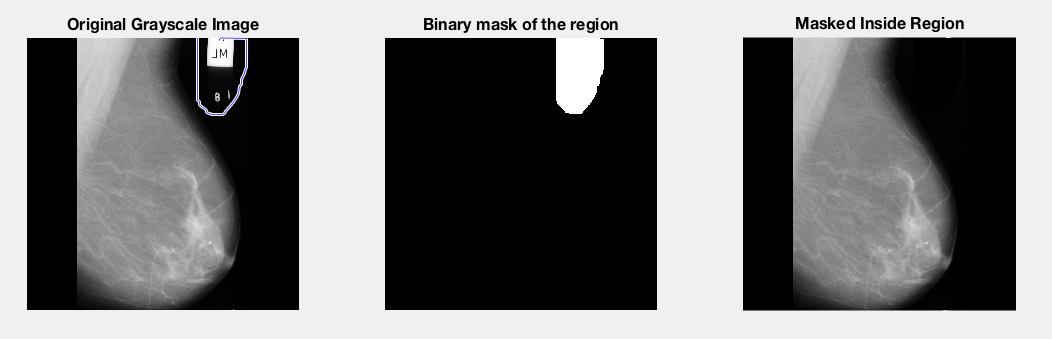
\includegraphics[scale=0.3]{Chapter2/technical-img/draw-to-remove.png}
  \caption{Image depicting the steps taken to remove medical markers from a scan.}
  \label{fig:remove-marker}
\end{figure}
